\section{Recommender Systems} \label{sec:recommender-systems}


Recommender systems are the subject of extensive research and have found wide-ranging applications in various domains, from e-commerce to entertainment and beyond \cite{RicciRecommenderSystems2015,AdomaviciusNextGeneration2005}. The fundamental objective of these systems is to predict preferences by learning from the past behavior of a user and the behavioral patterns of similar users.
In comparison to traditional keyword-centric search engines, recommender systems have proven to be more effective and reliable in drawing meaningful knowledge from large datasets \cite{BaiScientificPaper2020}.


\subsubsection*{Types of Recommender Systems}

Recommender systems can be classified into several categories based on their underlying algorithms and methodologies. The primary types encompass \ac{CF}, \ac{CBF}, and hybrid systems. Content-based techniques propose items that are similar to the ones a user has previously expressed interest in, while collaborative techniques recommend items that are favored by users with similar preferences \cite{BurkeHybridRecommender2002}.

According to a comprehensive survey conducted by Beel et al. \cite{BeelResearchpaperRecommender2016}, \ac{CBF} is the most commonly applied approach in research paper recommender systems, used in 55\% of the surveyed articles, while \ac{CF} was utilized in only 18\% of the articles reviewed.
The following sections introduce \ac{CF}, \ac{CBF}, and hybrid systems in more detail.


\subsection{Collaborative Filtering} \label{sec:collaborative-filtering}

The underlying assumption of \acl{CF} \cite{GoldbergUsingCollaborative1992,ResnickGroupLensOpen1994} is that those who agreed in the past will agree in the future, and that preferences for one user can be inferred from the preferences of similar users \cite{BaiScientificPaper2020}.
The conventional approach of \ac{CF} is user-oriented, whereby the system identifies users whose rating patterns are similar to those of the active user and recommends items that these like-minded users have shown interest in \cite{RicciRecommenderSystems2015}. Despite its efficacy, this method encounters scalability issues as the user base expands. Additionally, it is vulnerable to fluctuations in user behavior over time \cite{SarwarItembasedCollaborative2001}.

Sarwar et al. \cite{SarwarItembasedCollaborative2001} suggest item-based \ac{CF} to address the challenge of scalability.
This method operates by comparing items as opposed to users. It identifies correlations between different items based on the co-occurrence of ratings across users. Once these relationships have been established, the system can generate recommendations for a user based on their previous ratings of items. This method offers better scalability as the growth rate of items typically lags behind that of users, and it is also more robust to change since items do not exhibit changes in their behavior over time as it is the case with users.

Agarwal et al. \cite{AgarwalResearchPaper2005} propose a clustering approach to \ac{CF} to handle sparse, high-dimensional data. Their method, called Subspace Clustering Based Analysis (SCuBA), maps users to specific subspaces where similar browsing behavior is identified. Each subspace represents a specific user behavior, and users are assigned to the subspace that best matches their behavior. Recommendations are made based on popular items in the user's assigned subspace.

\ac{CF} has been effectively applied in many practical scenarios and fundamentally contributes to the success of many high-profile companies.
For instance, the Netflix Prize competition was designed to enhance the company's \ac{CF} algorithm \cite{KorenMatrixFactorization2009}. \ac{CF} is also employed by YouTube to recommend videos \cite{DavidsonYouTubeVideo2010,CovingtonDeepNeural2016} and by Amazon to suggest products \cite{LindenAmazonCom2003}.


\subsection{Content-Based Filtering} \label{sec:content-based-filtering}

\acl{CBF} methods utilize item features to generate recommendations. These methods propose items that are similar to the ones the user has previously shown interest in \cite{RicciRecommenderSystems2015}. The primary assumption in \ac{CBF} is that users will be attracted to items that resemble those they have previously liked \cite{BaiScientificPaper2020}.

Similar to \ac{CF}, \ac{CBF} also adopts two main forms: user-based and item-based \cite{BurkeHybridRecommender2002}. User-based \ac{CBF} recommends items based on the user's profile and their past behavior. Conversely, item-based \ac{CBF} generates recommendations based on similarities between items \cite{PazzaniContentBasedRecommendation2007}.
For example, a user-based \ac{CBF} system for academic papers may recommend a paper based on the user's previous ratings of similar papers. An item-based \ac{CBF} system, on the other hand, may recommend a paper based on the paper's similarity in topics, authors, or citations to other papers the user has previously rated.

\subsubsection*{Comparison of \acl{CF} and \acl{CBF}}

Both \ac{CF} and \ac{CBF} have their strengths and weaknesses.
By focusing on user-similarity rather than item-similarity, \ac{CF} can offer serendipitous recommendations \cite{BreitingerAcademicLiterature2023}. For instance, a user may be recommended a paper outside his research scope but which is highly rated by other users with similar interests. However, \ac{CF} is hindered by the cold-start problem, where new users or new items have no ratings and thus cannot be recommended \cite{DeyCollaborativeFiltering2021}. One approach to addressing the cold-start problem is to use \emph{implicit} feedback, such as the number of times a user has viewed an item \cite{HuCollaborativeFiltering2008} or the number of pages a user has read from a document as a proxy for the user's preference \cite{YangCARESRankingoriented2009}.

Conversely, \ac{CBF} allows for user-based personalization since it relies on the user's profile and past behavior. It is also not affected by the cold-start problem since it can recommend items based on their features alone \cite{DeyCollaborativeFiltering2021}. Further, \ac{CBF} requires less preliminary categorization work \cite{BreitingerAcademicLiterature2023} since user models can be created automatically. However, \ac{CBF} is highly dependent on the quality of the item features. For instance, if the item features are not sufficiently descriptive, the system may not be able to generate accurate recommendations. Further, \ac{CBF} tends to propose items that are similar to those the user has already rated, potentially limiting the diversity of the recommendations \cite{DeyCollaborativeFiltering2021,BurkeHybridRecommender2002}.

Ricci et al. \cite{RicciRecommenderSystems2015} suggest that \ac{CBF} is preferable when there's sufficient information about the items but less information about the users, whereas \ac{CF} is more useful in situations with abundant user information but limited item details.


\subsection{Hybridization Techniques} \label{sec:hybridization-techniques}

Hybrid recommender systems that combine \ac{CF} and \ac{CBF} can offer more accurate and diverse recommendations than either \ac{CF} or \ac{CBF} alone by addressing the limitations of each approach.
They can better address the cold-start problem than pure \ac{CF} systems and offer more diverse recommendations than pure \ac{CBF} systems \cite{BurkeHybridRecommender2002}.

Hybrid recommenders can be designed in several ways. Burke \cite{BurkeHybridRecommender2002} presents a classification of hybrid recommendation techniques, categorizing them into seven types: weighted, mixed, switching, feature combination, feature augmentation, cascade, and meta-level.
These techniques can be further classified into two categories: In \emph{weak} hybridization techniques, the primary technique remains dominant whereas in \emph{true} hybridization techniques, the two techniques equally contribute to the final recommendations \cite{BreitingerAcademicLiterature2023,BurkeHybridRecommender2002,BurkeHybridWeb2007}.
\ac{CBF} approaches commonly rely on the feature augmentation technique by using global relevance attributes such as citation counts, the article recency or the number of affiliations to rank candidate recommendations \cite{BreitingerAcademicLiterature2023}.

This thesis focuses on weak form of hybridization: the \emph{cascade} pattern. The cascade strategy uses a sequential approach: The first recommender generates a candidate list of recommendations, while the second recommender refines and re-ranks these recommendations \cite{BurkeHybridRecommender2002,chiangTypesHybrid2021} as illustrated in \Cref{fig:cascade}.
This method contrasts with parallel approaches, such as the weighted hybrid strategy, where both recommenders contribute to the final recommendation ranking and the impact of each recommender is controlled by a weighting factor \cite{BurkeHybridRecommender2002}.

\begin{figure}[ht]
    \centering
    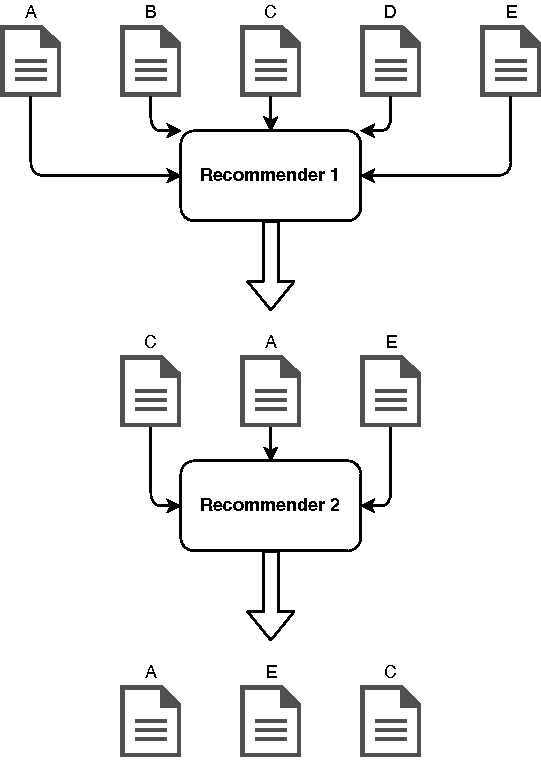
\includegraphics[width=0.5\textwidth]{diagrams/cascade.pdf}
    \caption[Cascade Hybridization Strategy]{The cascade hybridization strategy. Papers A - E represent candidate papers from the dataset. Recommender 1 generates a sorted candidate list of recommendations with Paper C as the top recommendation. The second recommender then refines and re-ranks the candidate list, resulting in Paper A as the top recommendation.}
    \label{fig:cascade}
\end{figure}

The primary motivation for using the cascade strategy in this thesis is its effect on the computational complexity of the hybrid system. In contrast to parallel techniques where both recommenders process the entire dataset, the cascade approach can significantly reduce the computational requirements by only requiring the first recommender to process the whole dataset. The second recommender only needs to process the candidate list generated by the first recommender, which is typically much smaller in size.
Therefore, the size of the candidate list can be seen as a hyperparameter with two responsibilities:

\begin{enumerate}
    \item It determines the computational effort for the second recommender. The larger the candidate list, the more documents have to be processed and re-ranked by the second recommender.
    \item It controls the impact of each recommender on the final recommendation ranking. If the candidate list is very large, the first recommender only excluded a small number of documents and the hybrid system heavily relies on the second recommender. Conversely, if the candidate list is very small, the first recommender already significantly reduced the set of potential recommendations and the second recommender has less impact on the final recommendation ranking.
\end{enumerate}


\subsection{Academic Paper Recommendation}

In the context of academic papers, \emph{users} can be conceptualized as researchers and \emph{items} as papers. However, the direct application of \ac{CF} to academic papers presents challenges due to the sparsity of the user-item matrix and the dynamic nature of user interests.

For academic papers, the user-item matrix which denotes interactions between users and items is frequently sparse. Unlike in broader fields such as movies or books, where a large number of individuals may interact with the same item, the audience for academic papers is typically more specific and smaller \cite{AgarwalResearchPaper2005}. This leads to fewer overlaps in the papers that researchers read, thereby making it difficult to form user groups based on shared interests - a fundamental element of \ac{CF}.
Alluding to the cold-start problem, new papers that have not been rated by any researchers cannot be recommended \cite{BreitingerAcademicLiterature2023}. Further, the continual change of academics in their research focus and reading patterns complicates the use of \ac{CF} in academic paper recommendation \cite{RoySystematicReview2022}.

When comparing the effectiveness of \ac{CF} and \ac{CBF} in the context of academic paper recommendation, the results are ambiguous \cite{BeelResearchpaperRecommender2016}.
Several studies have reported \ac{CBF} to outperform \ac{CF} for paper recommendation, while others have found the opposite to be true. Beel et al. \cite{BeelResearchpaperRecommender2016} suggest three potential reasons for these inconsistencies: limitations in the evaluations, a lack of detailed descriptions of the algorithms used, and different implementations of the same recommendation approaches leading to varying results.

This is where hybrid recommender systems have shown promise. By merging \ac{CF} and \ac{CBF}, hybrid systems can deliver more robust and flexible recommendations for academic papers \cite{BaiScientificPaper2020,SugiyamaExploitingPotential2013}. For instance, Kanakia et al. \cite{KanakiaScalableHybrid2019} combine co-citation analysis and content-based approaches in their system, leveraging the strengths of both methods. In the co-citation approach, papers that are often cited together are assumed to be similar. In the content-based approach, the text content of papers is analyzed to find similar papers. The hybridization enables the system to balance paper novelty (discovering new and lesser-known papers) against authority (recommending highly-cited and influential papers).

\Cref{sec:citation-analysis} and \Cref{sec:semantic-analysis} delve deeper into the two primary approaches employed in academic paper recommendation: citation analysis and semantic analysis. \Cref{sec:hybrid-recommenders-for-academic-papers} then explores the application of hybrid recommender systems to paper recommendation.


\subsection{Evaluation of Recommender Systems} \label{sec:evaluation-of-recommender-systems}

\subsubsection*{Types of Evaluation}

Evaluating the performance of recommender systems is an essential step in their development and deployment. The three prevalent types of evaluations include offline evaluations, online evaluations, and user studies \cite{BeelComparisonOffline2015}. Offline evaluations involve assessing the system's performance using pre-gathered data, while online evaluations test the system in a live setting with actual users capturing real-time user behavior.
User studies, on the other hand, involve detailed analyses of user interactions with the system, often involving user feedback and surveys. In this way, they can provide insights into user preferences and experiences.

However, the outcomes from these evaluation methodologies may not always align. For instance, a system that performs well in offline evaluations may not deliver the same performance in online evaluations or user studies \cite{BeelComparisonOffline2015}. Offline evaluations are based on historical data and may not accurately reflect current or future user behavior. Moreover, offline evaluations often rely on implicit feedback (e.g., click-through rates), which may not fully capture user satisfaction or user preferences.

Despite these limitations, offline evaluations remain popular as they can be used to compare different approaches quickly and inexpensively.
Yet, for a more accurate and comprehensive understanding of a recommender system's performance, Beel and Langer \cite{BeelComparisonOffline2015} suggest that offline evaluations should be complemented with online evaluations and user studies.

\subsubsection*{Evaluation Metrics}

Accuracy-based metrics are popular due to their straightforward quantification and interpretation. These include the Root Mean Squared Error, Precision, Recall, F1 score, and AUC \cite{SilveiraHowGood2019,BaiScientificPaper2020,RicciRecommenderSystems2015}.

However, there are variations of these metrics that are more suited to evaluating recommender systems, including \ac{Patk}, \ac{Ratk}, \ac{AP}, \acf{MAP}, \ac{MRR}, \ac{DCG}, and \ac{NDCG} \cite{SilveiraHowGood2019}.

\ac{Patk} is computed as the number of relevant items in the top-k recommendations divided by k \cite{BaiScientificPaper2020}. Mathematically, this is expressed as:

\begin{align}
    P@k = \frac{1}{k} \sum_{i=1}^{k} \mathbbm{1}(i \text{ is relevant}) = \frac{\# \text{ of recommended relevant items}}{k} \label{eq:precision-at-k}
\end{align}

where $\mathbbm{1}(i \text{ is relevant})$ is an indicator function that equals 1 if the $i^{th}$ recommendation is relevant and 0 otherwise. \ac{Patk} is a suitable metric when the aim is to recommend a few high-quality items to the user, regardless of their ranking in the recommendation list.

On the other hand, \ac{Ratk} is the proportion of the relevant items that are included in the top-k recommendations \cite{BaiScientificPaper2020}. This is calculated as:

\begin{align}
    R@k = \frac{1}{m} \sum_{i=1}^{k} \mathbbm{1}(i \text{ is relevant}) = \frac{\# \text{ of recommended relevant items}}{m} \label{eq:recall-at-k}
\end{align}

where $m$ is the total number of relevant items. \ac{Ratk} is a more suited metric when the aim is to identify as many relevant items as possible in the top-k recommendations, regardless of their position and the total number of recommendations.

\ac{MAP} is an extension of the Precision metric that takes into account the order of the recommendations and is more suited for systems where ranking is crucial \cite{RinkMeanAverage2023,TaifiMRRVs2020,BaiScientificPaper2020}. Like \ac{Patk}, \ac{MAP} requires a binary classification of the recommendations as relevant or irrelevant.

For a set of queries, the \ac{MAP} is the mean of the \ac{AP}. The \ac{AP} for a single query is calculated as:

\begin{align}
    AP = \frac{1}{m} \sum_{k=1}^{n} P@k \cdot \mathbbm{1}(k \text{ is relevant}) \label{eq:average-precision}
\end{align}

where $n$ is the total number of recommendations and $m$ is the total number of relevant items. Then, \ac{MAP} is computed as:

\begin{align}
    MAP = \frac{1}{Q} \sum_{q=1}^{Q} AP_q \label{eq:mean-average-precision}
\end{align}

where $Q$ is the total number of queries and $AP_q$ is the \ac{AP} for the $q^{th}$ query. \ac{AP} and \ac{MAP} are particularly useful when the recommender system is expected to retrieve several relevant items and their ranks are important.

\ac{MRR} is another metric that considers the position of the relevant items, but only takes the first relevant item into account \cite{WikipediacontributorsMeanReciprocal2022,TaifiMRRVs2020,BaiScientificPaper2020}. \ac{MRR} is defined as:

\begin{align}
    MRR = \frac{1}{Q} \sum_{q=1}^{Q} \frac{1}{\text{rank}_q} \label{eq:mean-reciprocal-rank}
\end{align}

where $\text{rank}_q$ is the rank of the first relevant item for the $q^{th}$ query. \ac{MRR} is a suitable metric when the goal of the recommender system is to recommend the most relevant item as early as possible.

\ac{DCG} and its normalized form \ac{NDCG} consider the relevance of each item as well as their positions \cite{WikipediacontributorsDiscountedCumulative2022,TaifiMRRVs2020,BaiScientificPaper2020}. \ac{DCG} is calculated as:

\begin{align}
    DCG@k = \sum_{i=1}^{k} \frac{\text{rel}_i}{\log_2(i+1)} \label{eq:discounted-cumulative-gain}
\end{align}

where $\text{rel}_i$ is the relevance of the $i^{th}$ recommendation. The \ac{DCG} is then normalized by the ideal \ac{DCG} (IDCG), which is the \ac{DCG} value for the optimal recommendation list where all items are sorted by their relevance:

\begin{align}
    NDCG@k = \frac{DCG@k}{IDCG@k} \label{eq:normalized-discounted-cumulative-gain}
\end{align}

\ac{NDCG} is particularly useful when different items have different levels of relevance and they cannot be classified into binary categories (e.g., relevant or irrelevant).


\subsubsection*{Metrics Beyond Accuracy}

While accuracy-based metrics have dominated the evaluation of recommender systems, they overlook other important aspects that influence the quality of a recommender system. These include diversity, serendipity, novelty, and coverage \cite{KaminskasDiversitySerendipity2016,SilveiraHowGood2019,BaiScientificPaper2020}.
Diversity refers to the variety in the list of recommendations, serendipity to the element of surprise, novelty to the newness or unfamiliarity of the recommended items, and coverage to the proportion of items or users for which the system can generate recommendations.
Despite their significance, there is a scarcity of comprehensive research in these areas, which underscores the need for further exploration how alternative metrics can enhance the effectiveness and user experience of recommender systems \cite{SilveiraHowGood2019}.

Moreover, Bai et al. \cite{BaiScientificPaper2020} identify a growing demand for personalized, context-aware, and cross-domain recommendation systems to cater more effectively to diverse user needs.
Roy and Dutta \cite{RoySystematicReview2022} underscore that recommendations can be significantly improved by considering the context in which they are made. Contextual factors may include the time of day, the user's location, or even the user's mood. Incorporating these factors into recommender systems can help to tailor recommendations to the user's specific circumstances, thus improving the user experience.

In conclusion, there are several challenges in the field of recommender systems that need to be addressed in future research. The most prominent ones include dealing with the cold-start problem, handling the high dimensionality of data, managing the dynamic nature of user interests, and protecting user privacy in recommendation systems \cite{BaiScientificPaper2020,RicciRecommenderSystems2015,KanakiaScalableHybrid2019,RoySystematicReview2022}.
